\documentclass[notes]{beamer}
\usetheme{Rochester}

\usepackage{graphicx}
\usepackage{amsmath,amssymb}
\usepackage{ gensymb }

\title{Projects in Exoplanets}
\subtitle{TESS Lightcurve Photometry}
\author{Dina Sofia Mortensen \& Jesper Dam Knudgaard}
\institute{Stellar Astrophysics Centre, Aarhus University}
\date{January 18, 2019}

\begin{document}

\begin{frame}
\titlepage
\end{frame}

\section{Data Analysis}

\subsection{Initial Method}

\begin{frame}
\frametitle{Raw Data}
\centering
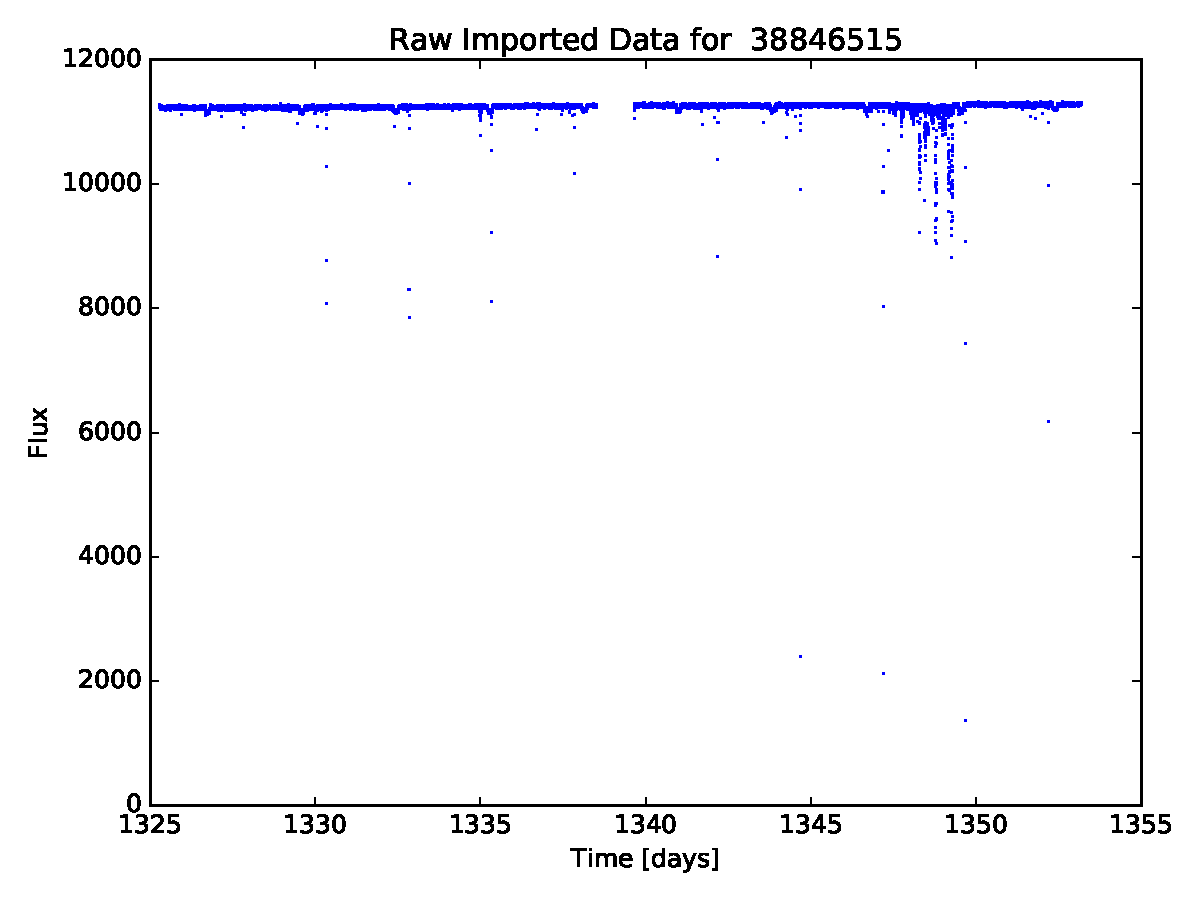
\includegraphics[width=0.9\textwidth]{../figures/2019-1-15_16:2:14_rawdata_TIC38846515.pdf}
\end{frame}

\begin{frame}
\frametitle{Normalization}
\centering
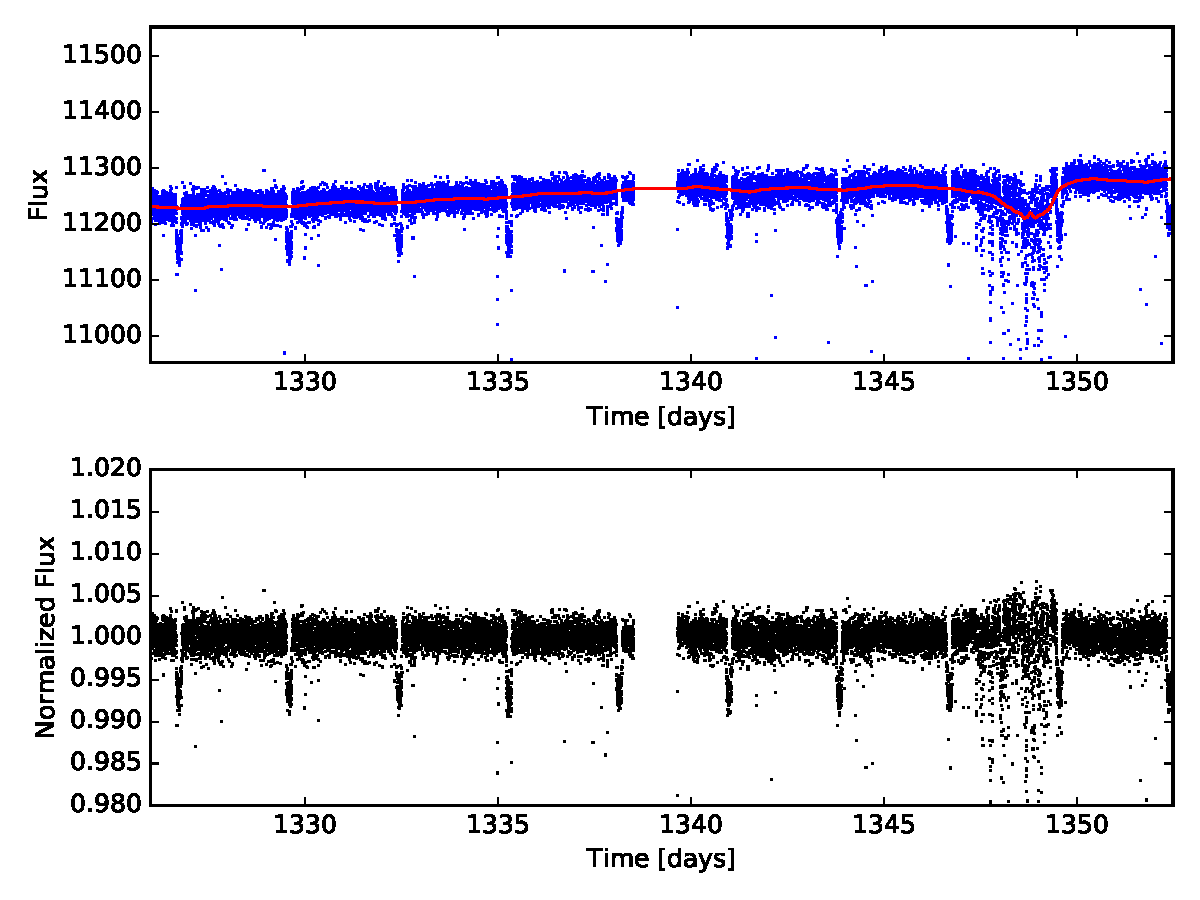
\includegraphics[width=0.9\textwidth]{../figures/2018-11-9_14:25:51_norm_curve0.pdf}
\end{frame}

\begin{frame}
\frametitle{Moving Median Filter}
\centering
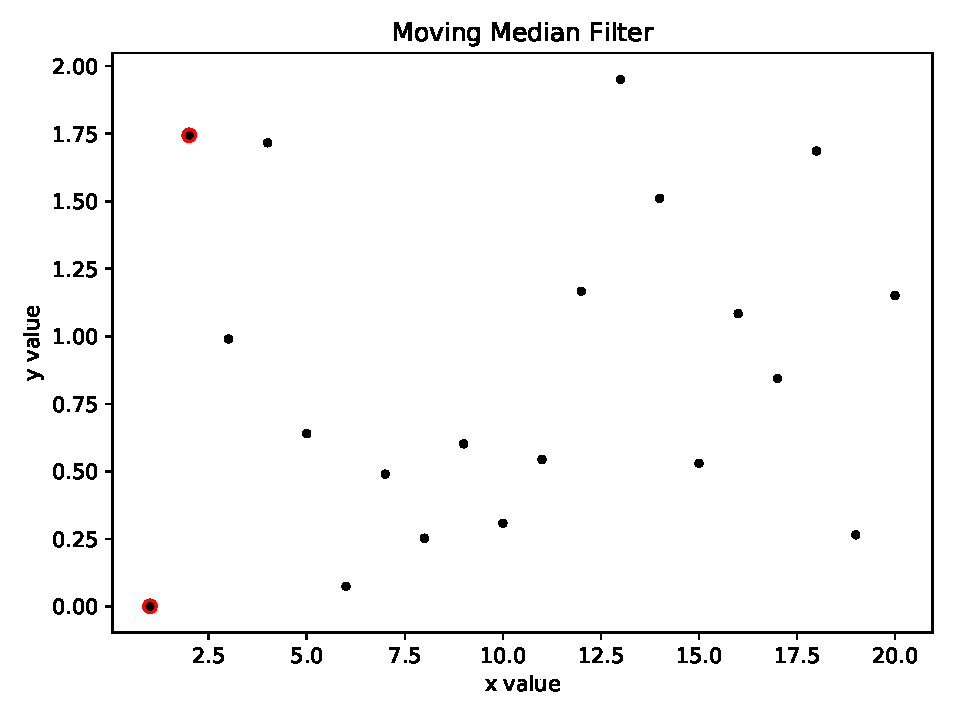
\includegraphics[width=0.9\textwidth]{../med_filt_dem_fig/med_filt_0.pdf}
\end{frame}

\begin{frame}
\frametitle{Moving Median Filter}
\centering
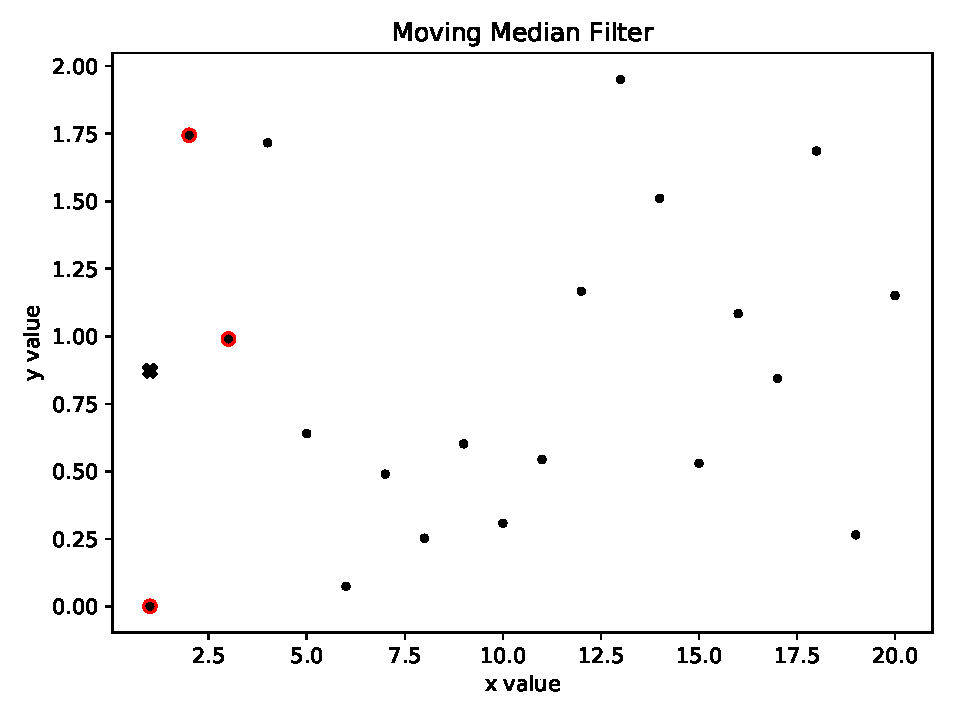
\includegraphics[width=0.9\textwidth]{../med_filt_dem_fig/med_filt_1.pdf}
\end{frame}

\begin{frame}
\frametitle{Moving Median Filter}
\centering
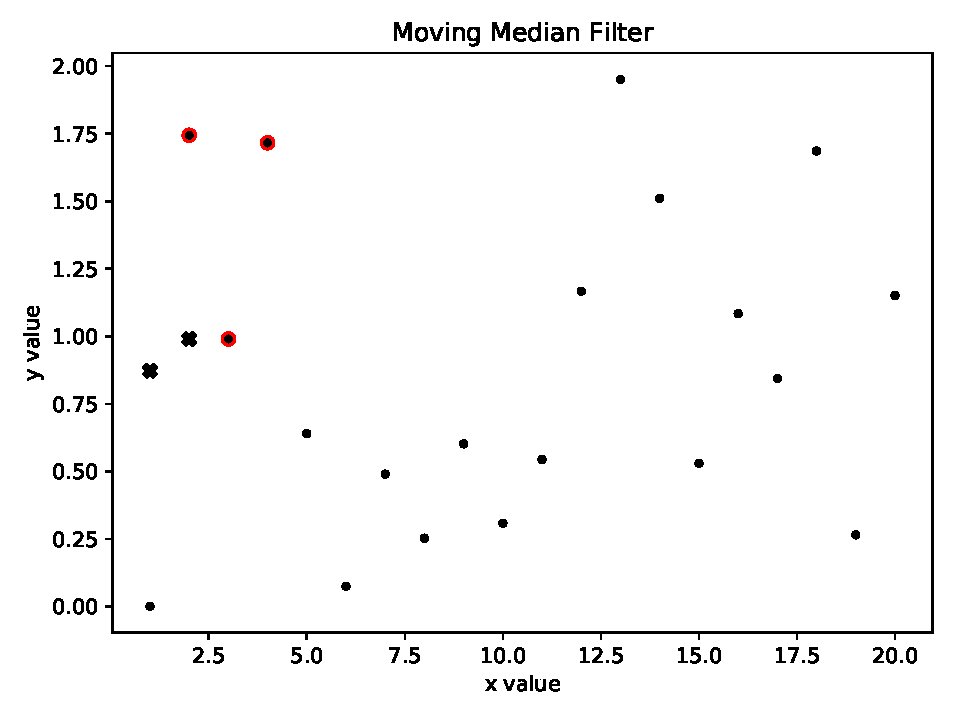
\includegraphics[width=0.9\textwidth]{../med_filt_dem_fig/med_filt_2.pdf}
\end{frame}

\begin{frame}
\frametitle{Moving Median Filter}
\centering
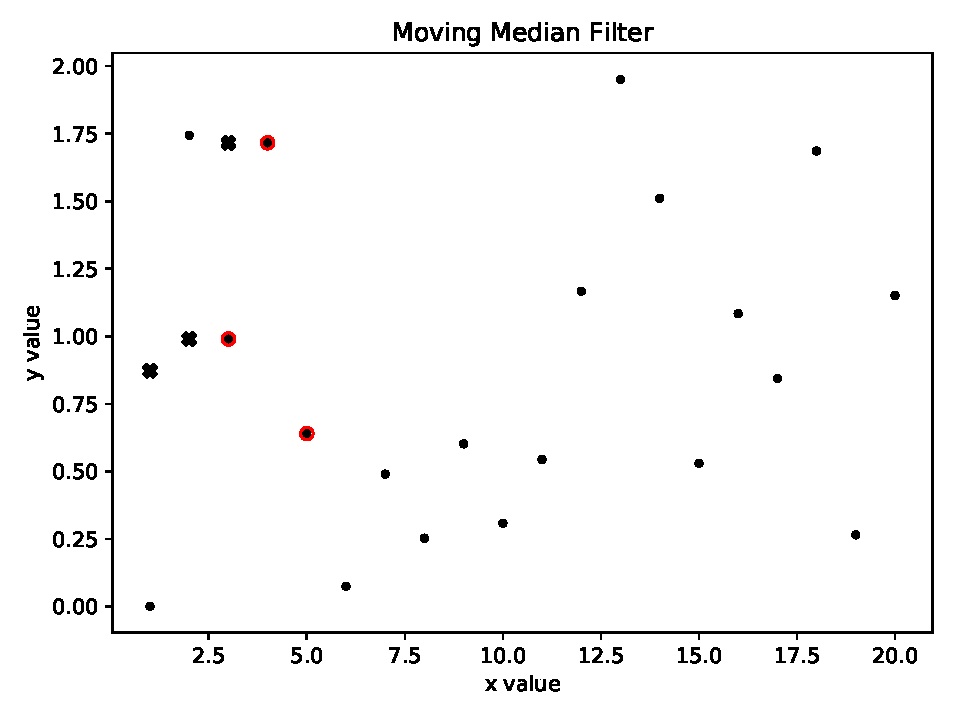
\includegraphics[width=0.9\textwidth]{../med_filt_dem_fig/med_filt_3.pdf}
\end{frame}

\begin{frame}
\frametitle{Moving Median Filter}
\centering
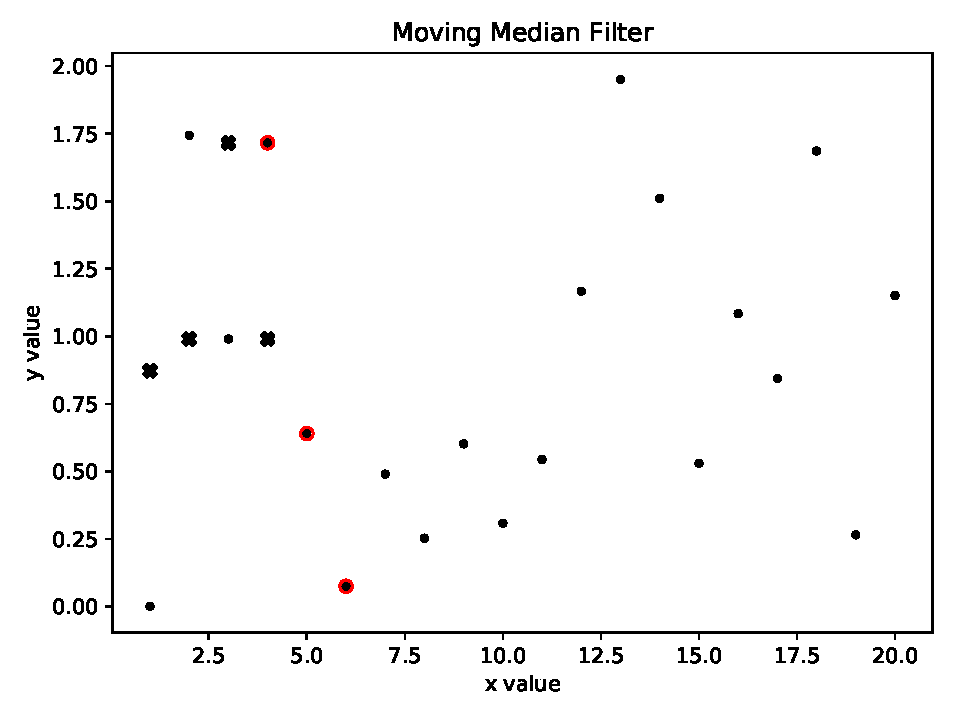
\includegraphics[width=0.9\textwidth]{../med_filt_dem_fig/med_filt_4.pdf}
\end{frame}

\begin{frame}
\frametitle{Moving Median Filter}
\centering
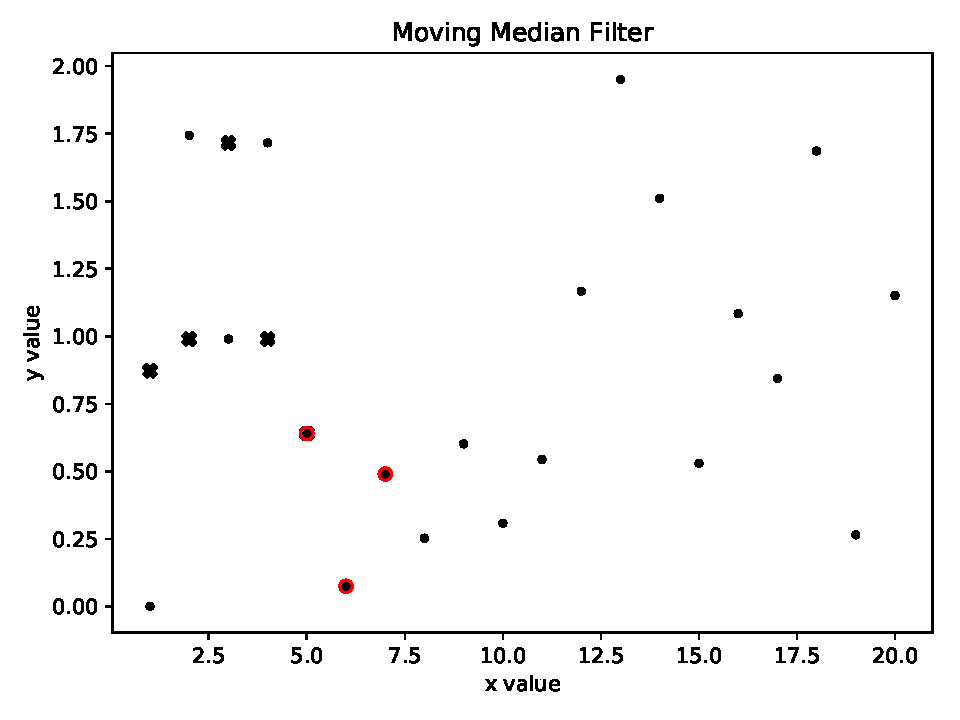
\includegraphics[width=0.9\textwidth]{../med_filt_dem_fig/med_filt_5.pdf}
\end{frame}

\begin{frame}
\frametitle{Interpolation}
\centering
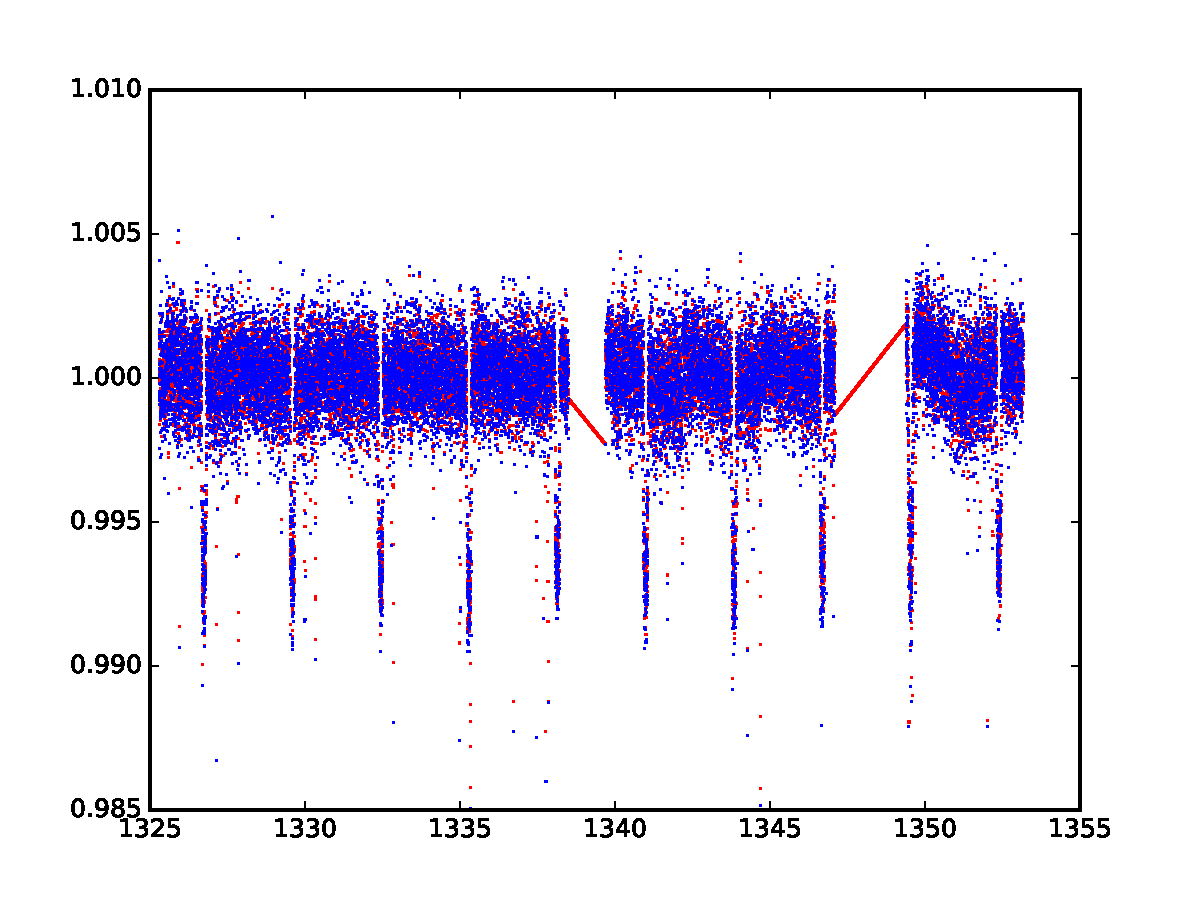
\includegraphics[width=0.9\textwidth]{../figures/2018-11-14_15:35:52_inter_curve0.pdf}
\end{frame}

\begin{frame}
\frametitle{Autocorrelation}
\centering
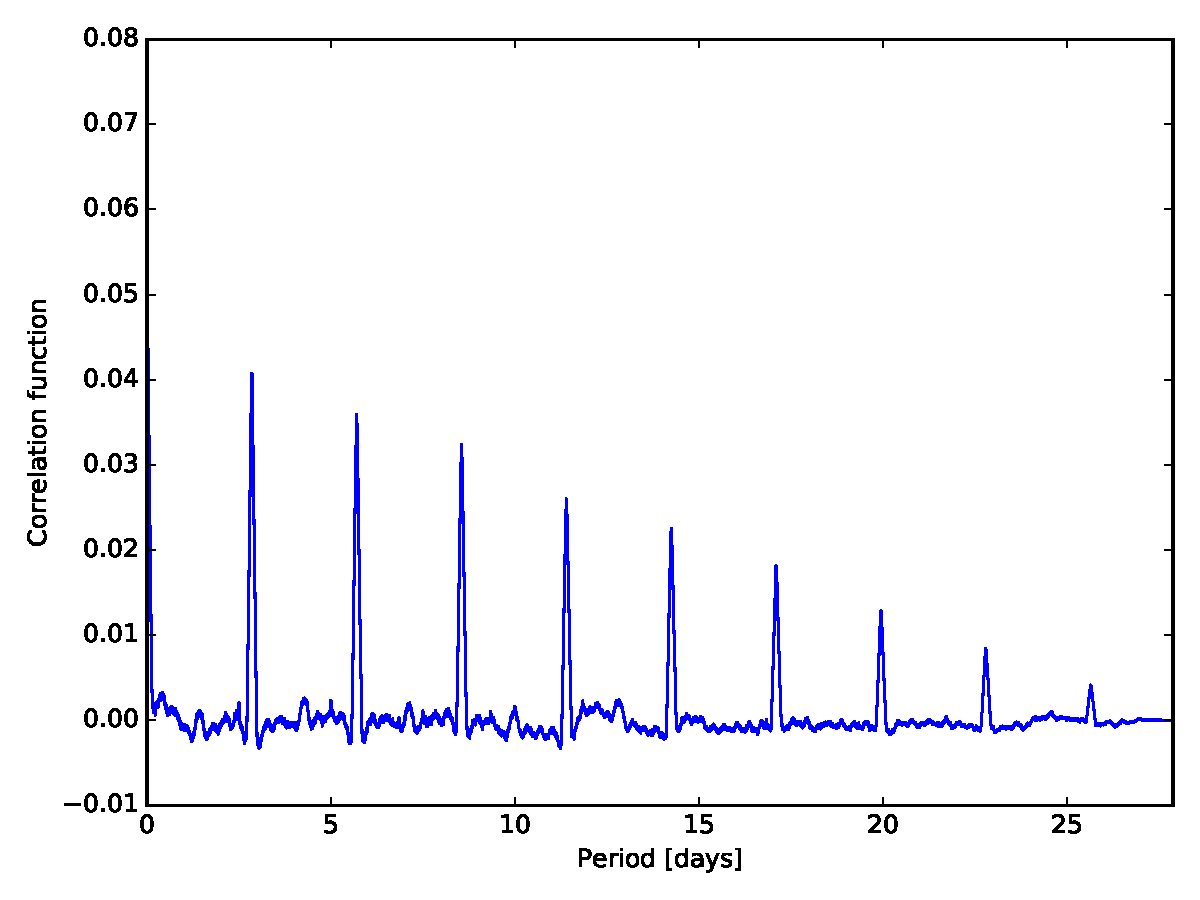
\includegraphics[width=0.9\textwidth]{../figures/2018-11-19_14:46:56_correlation_fig0.pdf}
\end{frame}

\begin{frame}
\frametitle{Autocorrelation + Peaks + Gaussian}
\centering
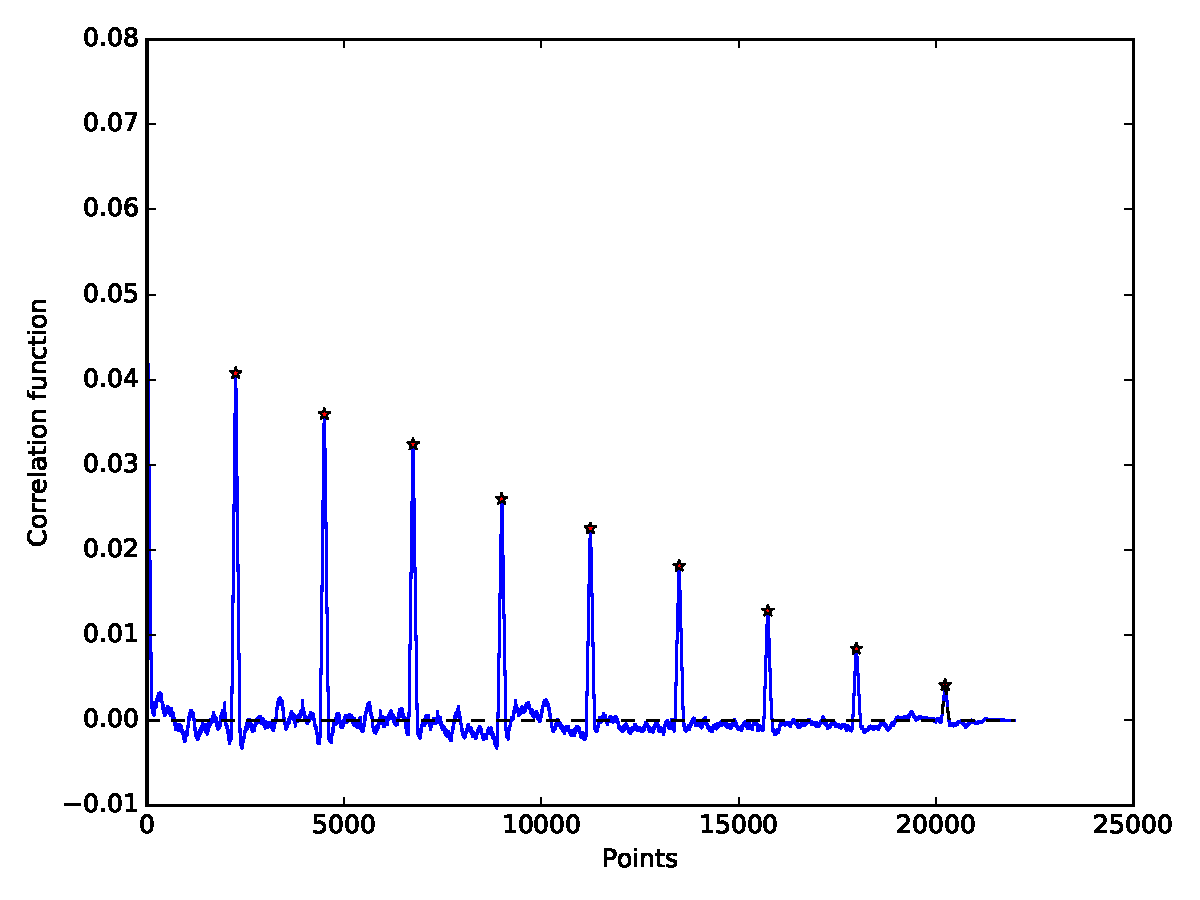
\includegraphics[width=0.9\textwidth]{../figures/2018-11-20_11:12:6_peaks_fig0.pdf}
\end{frame}

\begin{frame}
\frametitle{Folded Light Curve}
\centering
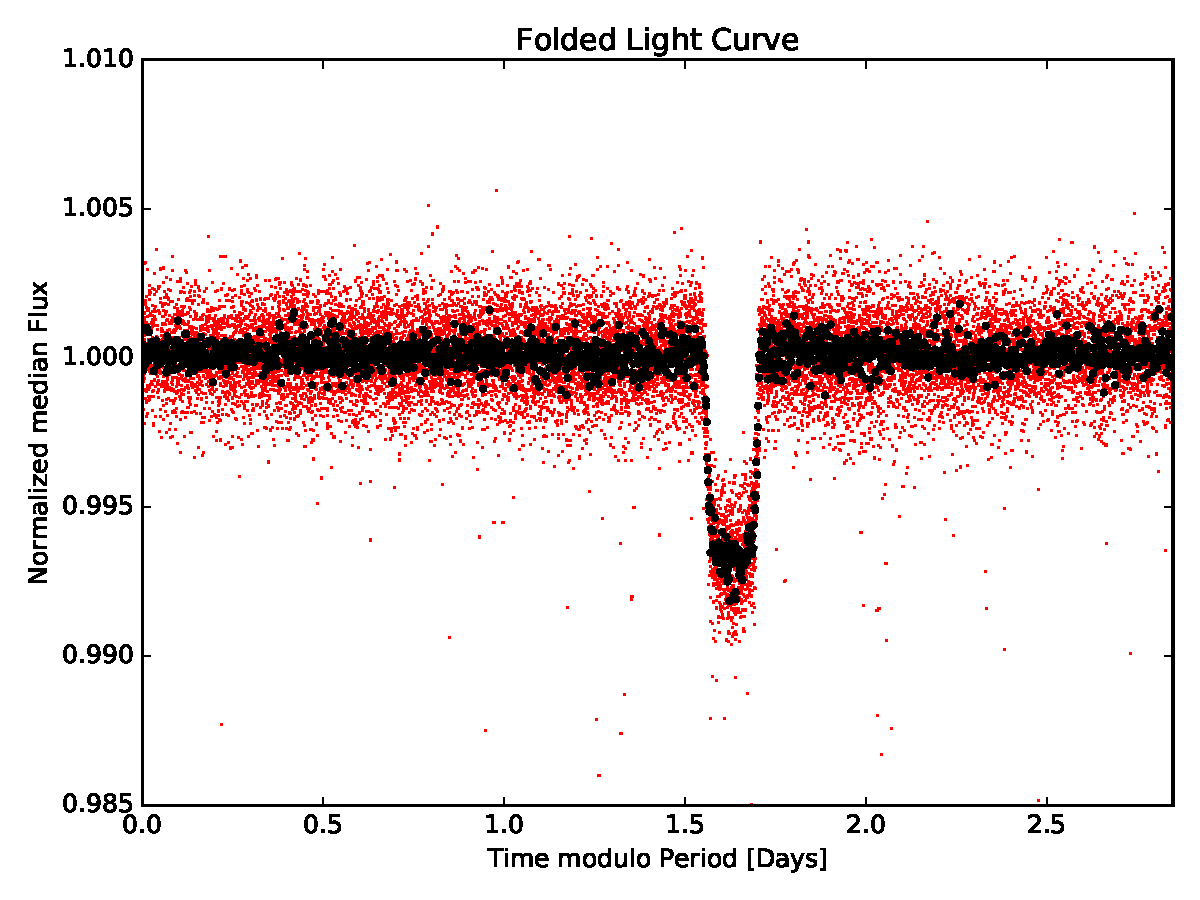
\includegraphics[width=0.9\textwidth]{../figures/2018-11-27_12:41:56_Folded0.pdf}
\end{frame}

\subsection{Improved Method}

\begin{frame}
\frametitle{Fine-mesh Moving Median Filter}
\centering
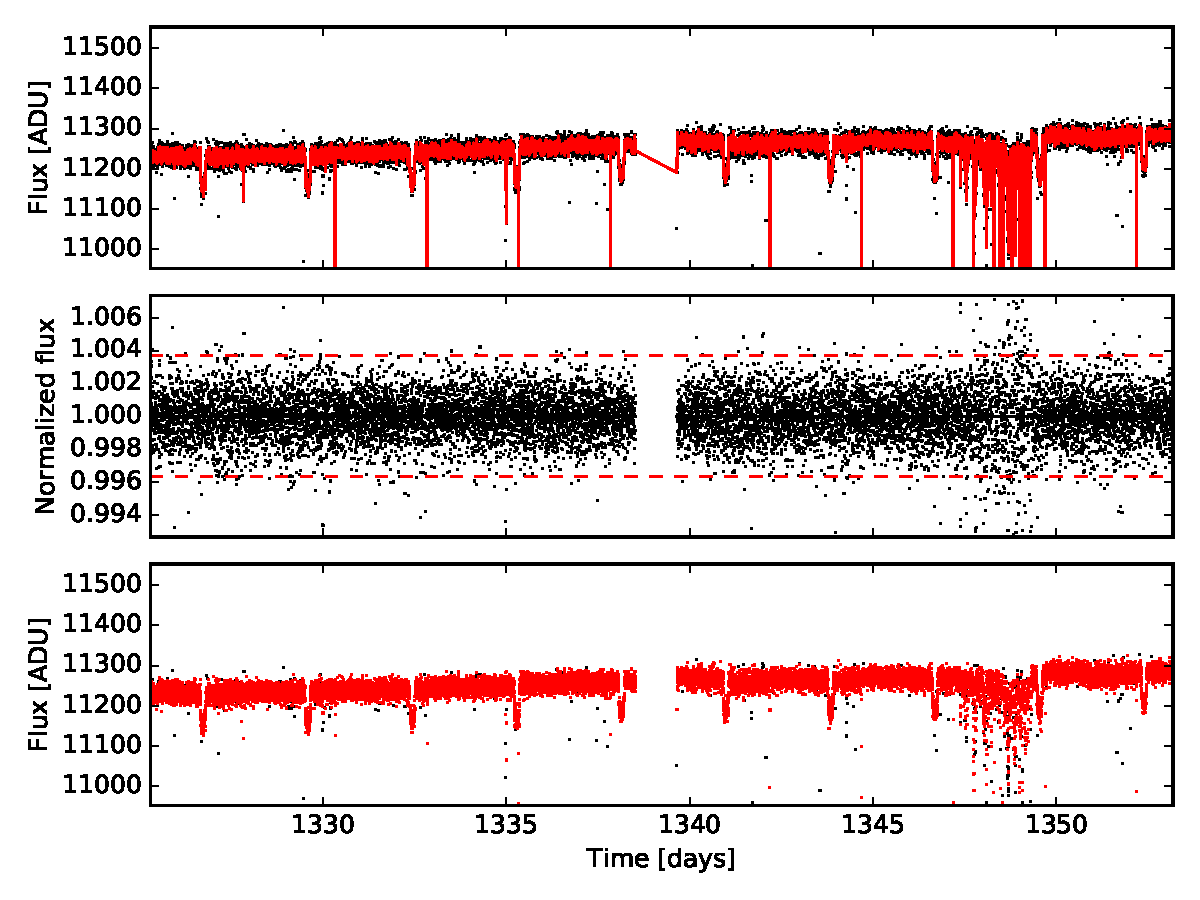
\includegraphics[width=0.9\textwidth]{../figures/2018-11-27_14:45:48_fine_mesh0.pdf}
\end{frame}

\begin{frame}
\frametitle{Fine-mesh Moving Median Filter}
\centering
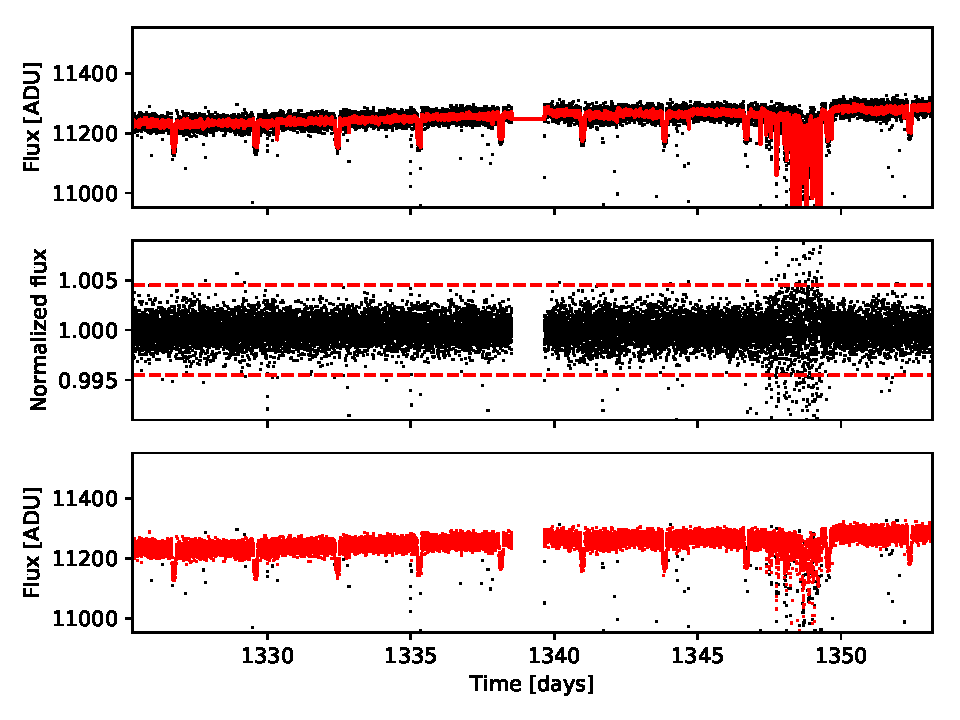
\includegraphics[width=0.9\textwidth]{../figures/2019-1-15_11:5:15_finemesh_TIC38846515.pdf}
\end{frame}

\begin{frame}
\frametitle{Normalization}
\centering
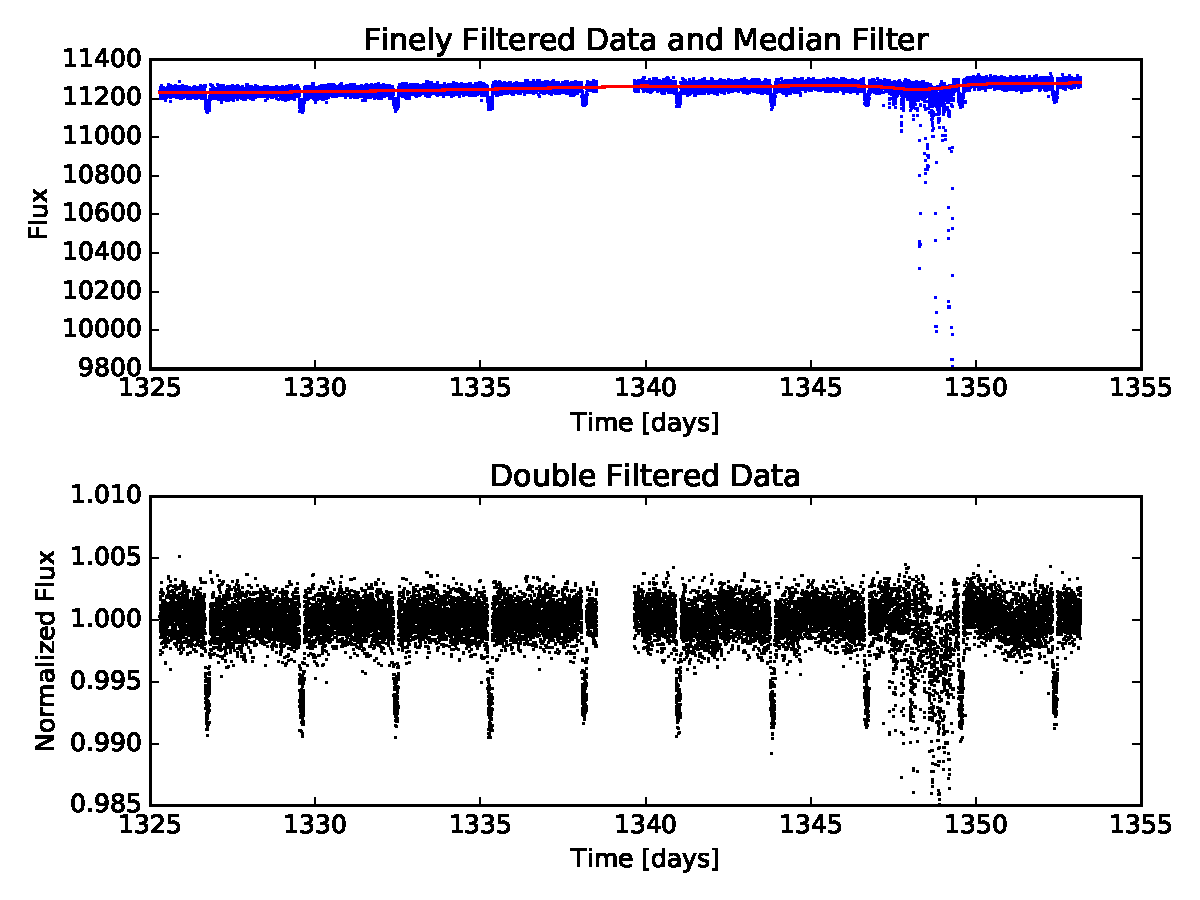
\includegraphics[width=0.9\textwidth]{../figures/2019-1-15_16:2:14_normcurve_lightcurve_TIC38846515.pdf}
\end{frame}

\begin{frame}
\frametitle{if $y[i]>1: y=1$}
\centering
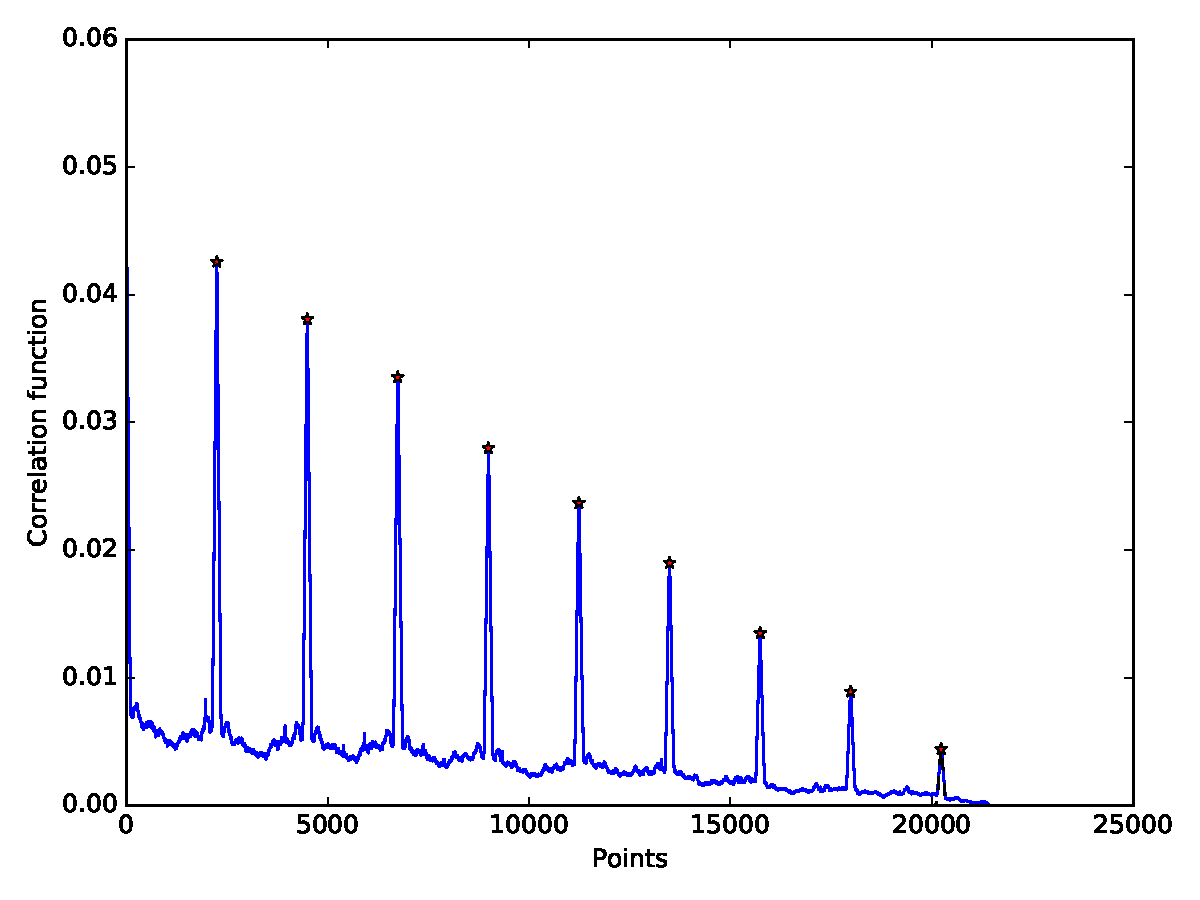
\includegraphics[width=0.9\textwidth]{../figures/2018-11-27_14:45:48_peaks_fig0.pdf}
\end{frame}

\begin{frame}
\frametitle{Interpolation Improvement}
\centering
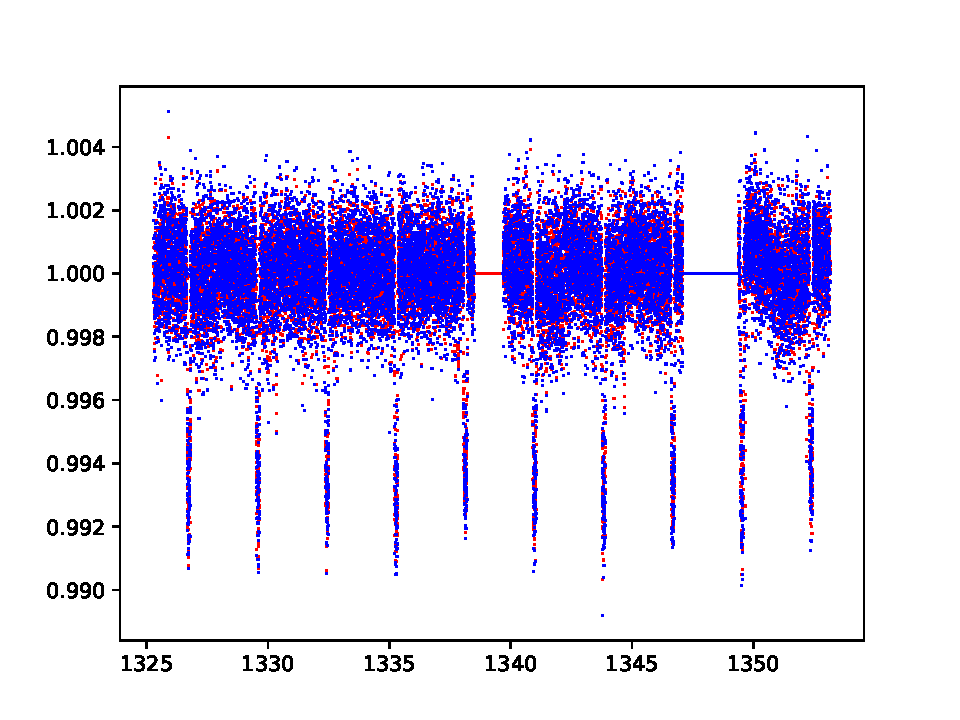
\includegraphics[width=0.9\textwidth]{../figures/2019-1-15_11:5:15_intercurve_TIC38846515.pdf}
\end{frame}

\begin{frame}
\frametitle{Normalized Correlation}
\centering
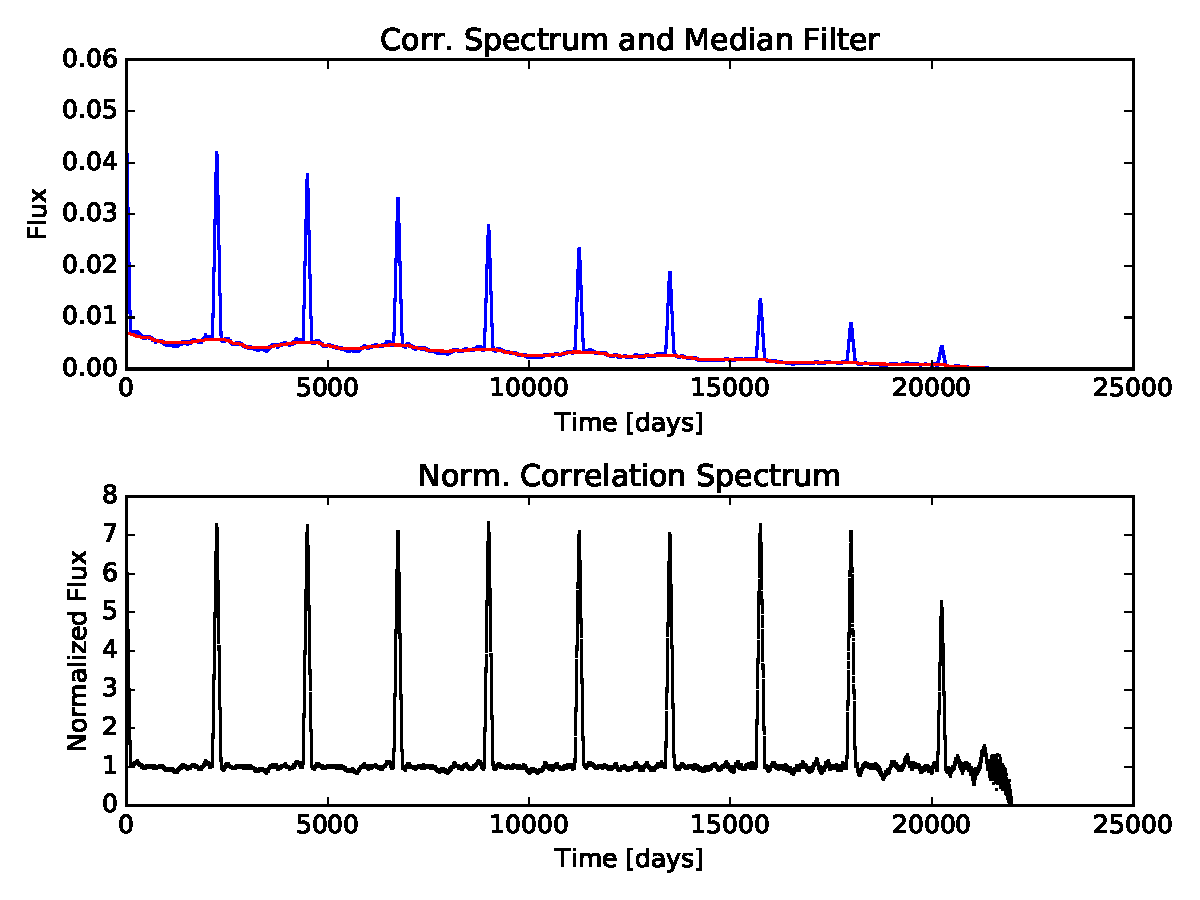
\includegraphics[width=0.9\textwidth]{../figures/2019-1-15_16:2:14_normcurve_correlation_TIC38846515.pdf}
\end{frame}

\begin{frame}
\frametitle{Fitting to All Peaks}
\centering
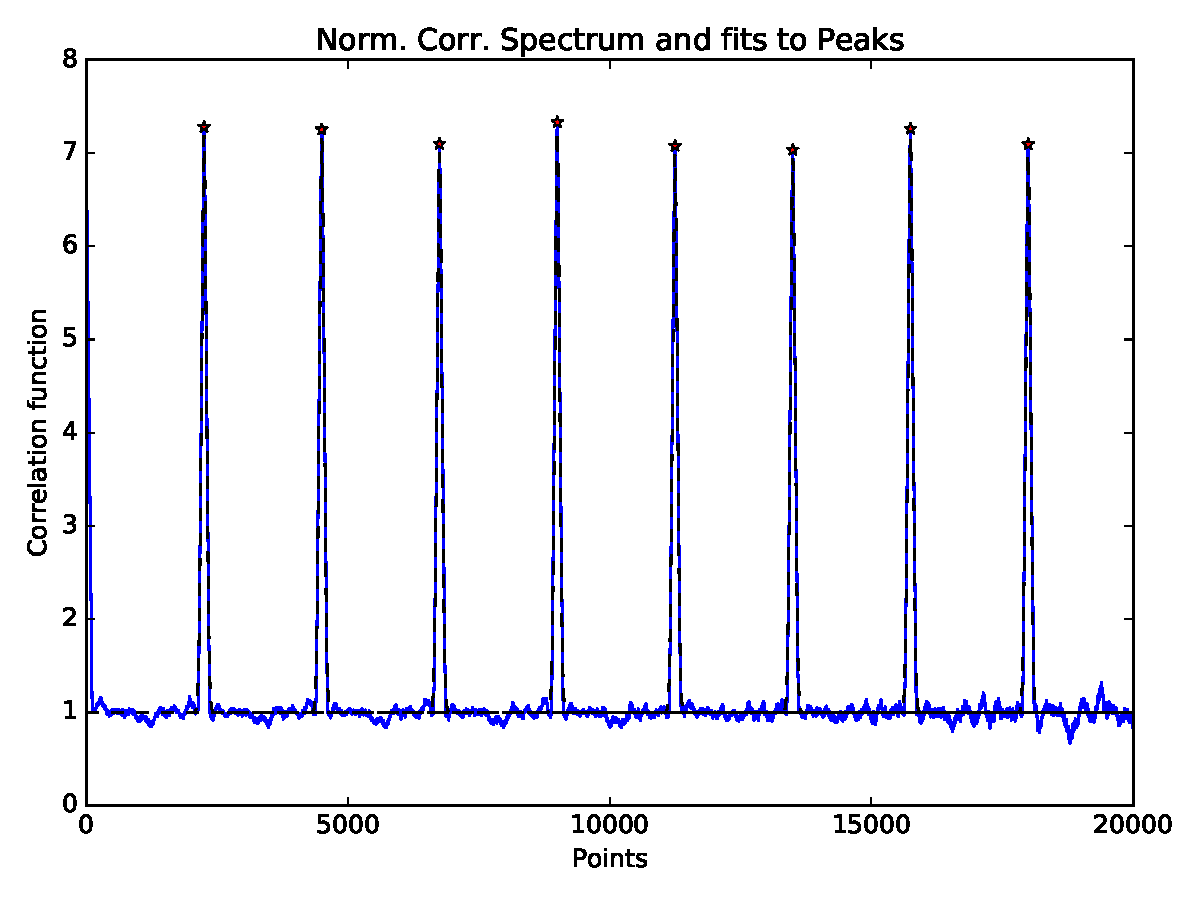
\includegraphics[width=0.9\textwidth]{../figures/2019-1-15_16:2:14_peaks_TIC38846515.pdf}
\end{frame}

\begin{frame}
\frametitle{Linear Fit to Period}
\centering
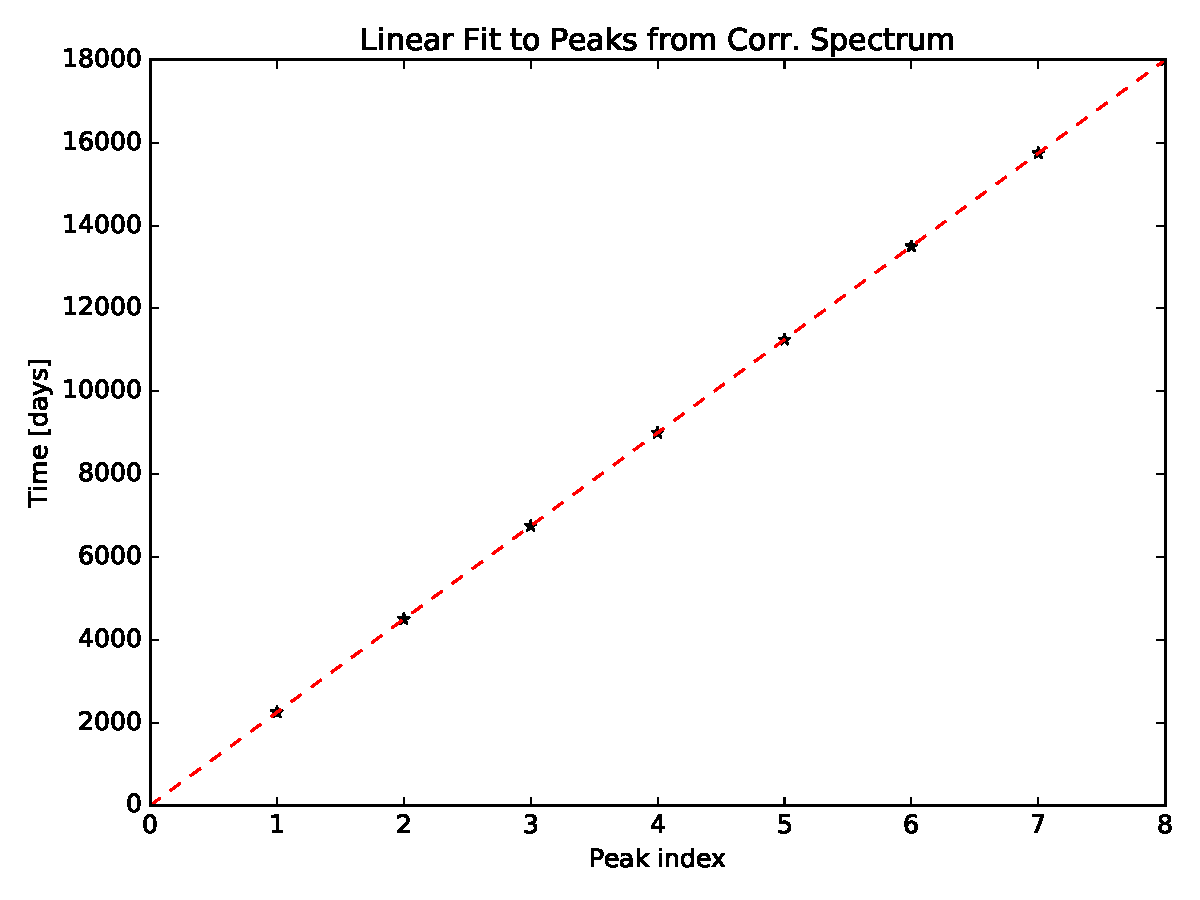
\includegraphics[width=0.9\textwidth]{../figures/2019-1-15_16:2:14_linear_fit_TIC38846515.pdf}
\end{frame}

\subsection{Results: Folded Light Curves}

\begin{frame}
\frametitle{TIC 38846515: Folded Light Curve}
\centering
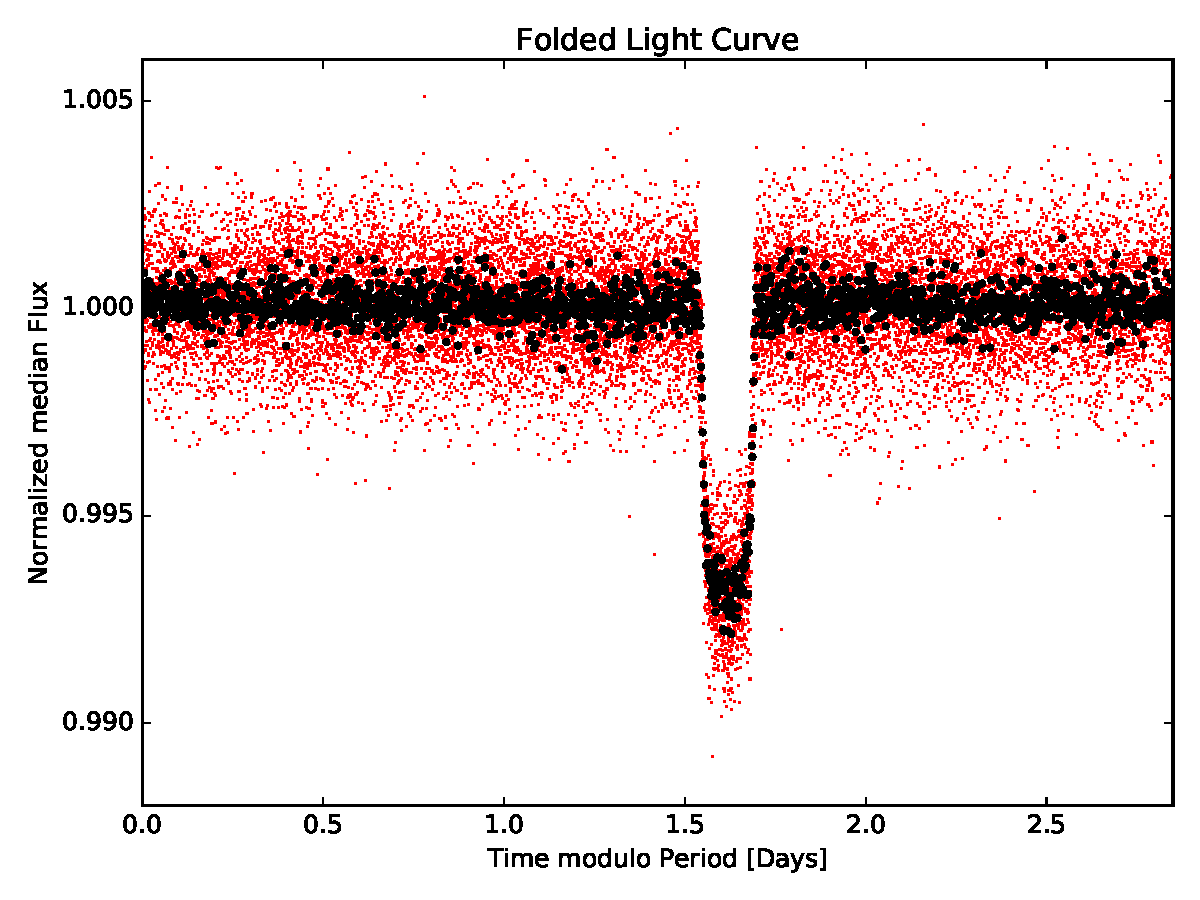
\includegraphics[width=0.9\textwidth]{../figures/2019-1-15_16:2:14_Folded_TIC38846515.pdf}
\end{frame}

\begin{frame}
\frametitle{TIC 76989773: Folded Light Curve}
\centering
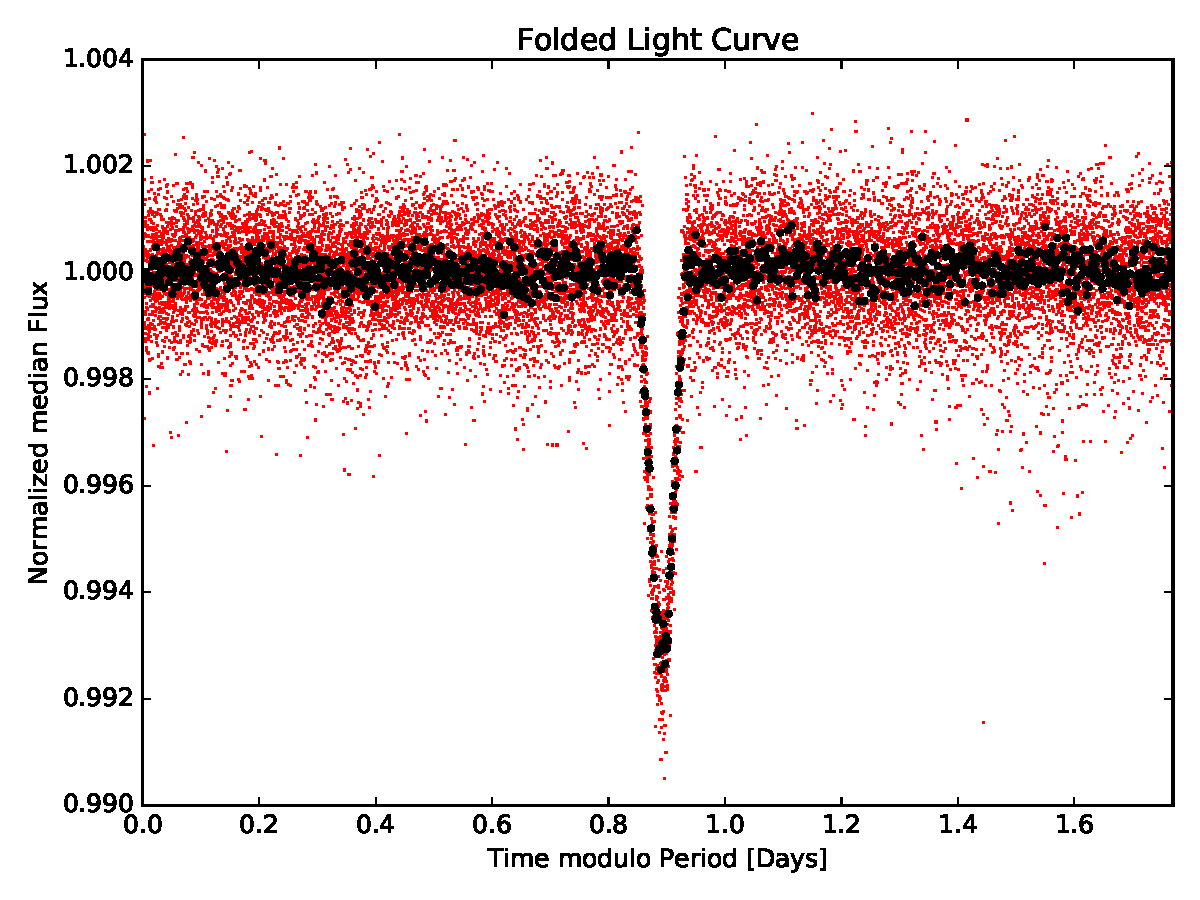
\includegraphics[width=0.9\textwidth]{../figures/2019-1-15_16:2:14_Folded_TIC76989773.pdf}
\end{frame}

\begin{frame}
\frametitle{TIC 201248411: Folded Light Curve}
\centering
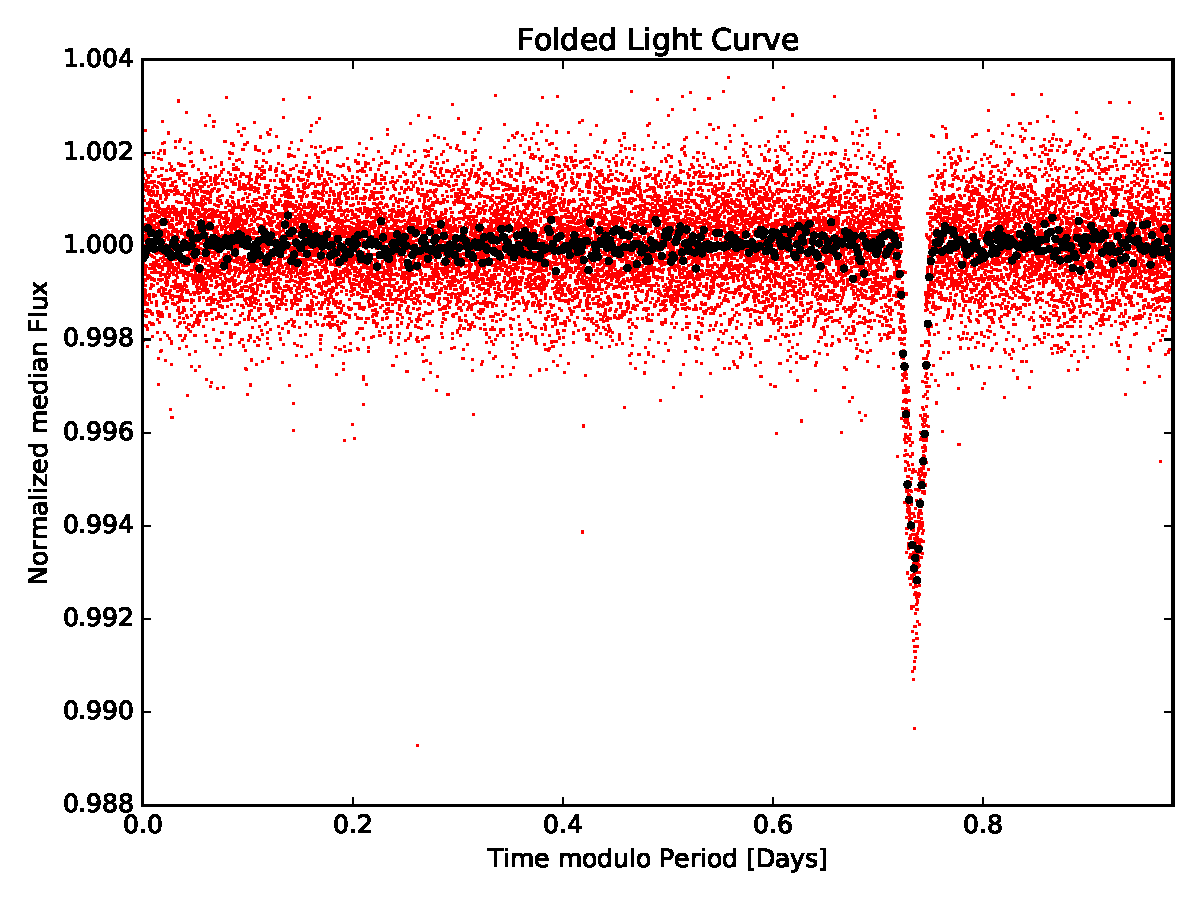
\includegraphics[width=0.9\textwidth]{../figures/2019-1-15_16:2:14_Folded_TIC201248411.pdf}
\end{frame}

\begin{frame}
\frametitle{TIC 29344935: Folded Light Curve}
\centering
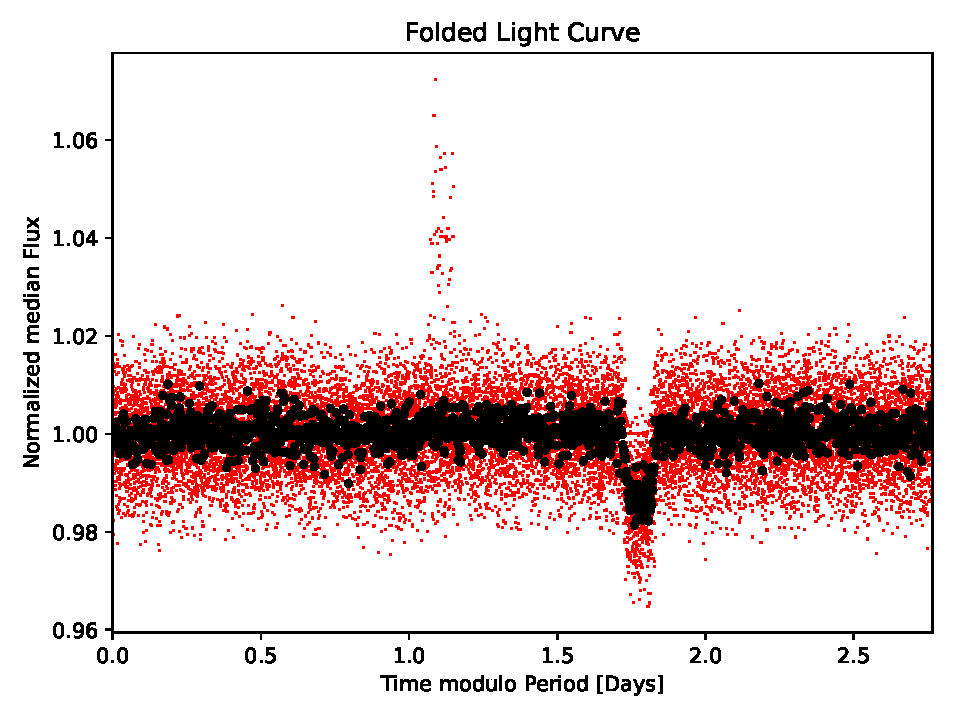
\includegraphics[width=0.9\textwidth]{../figures/2019-1-16_12:58:51_Folded_TIC29344935.pdf}
\end{frame}

\begin{frame}
\frametitle{TIC 25375553: Folded Light Curve}
\centering
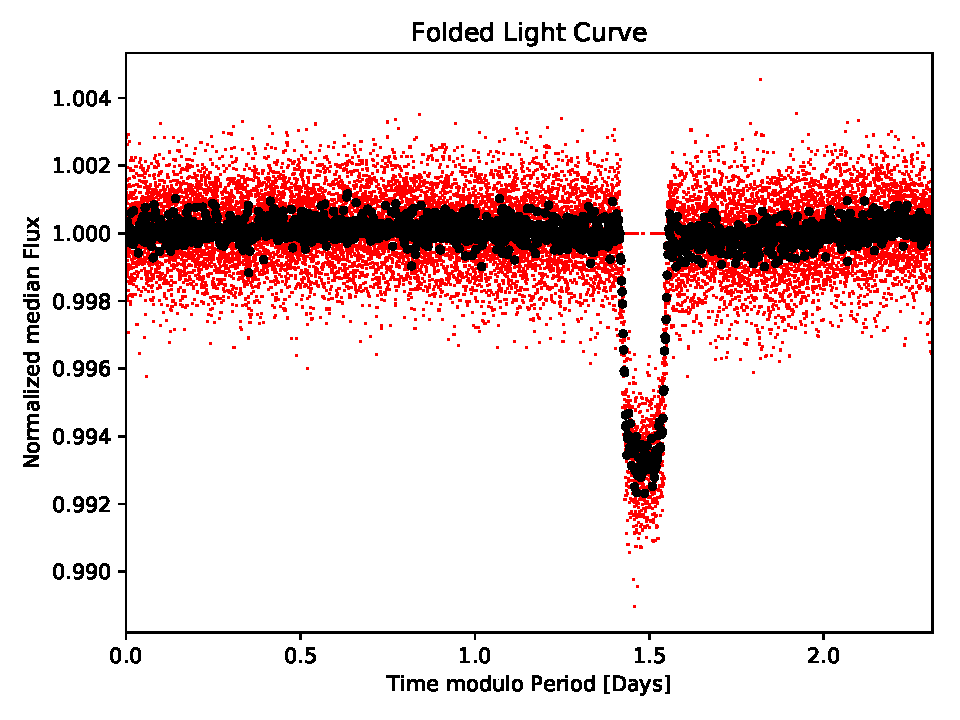
\includegraphics[width=0.9\textwidth]{../figures/2019-1-16_12:58:51_Folded_TIC25375553.pdf}
\end{frame}

\begin{frame}
\frametitle{TIC 25375553: Folded Light Curve}
\centering
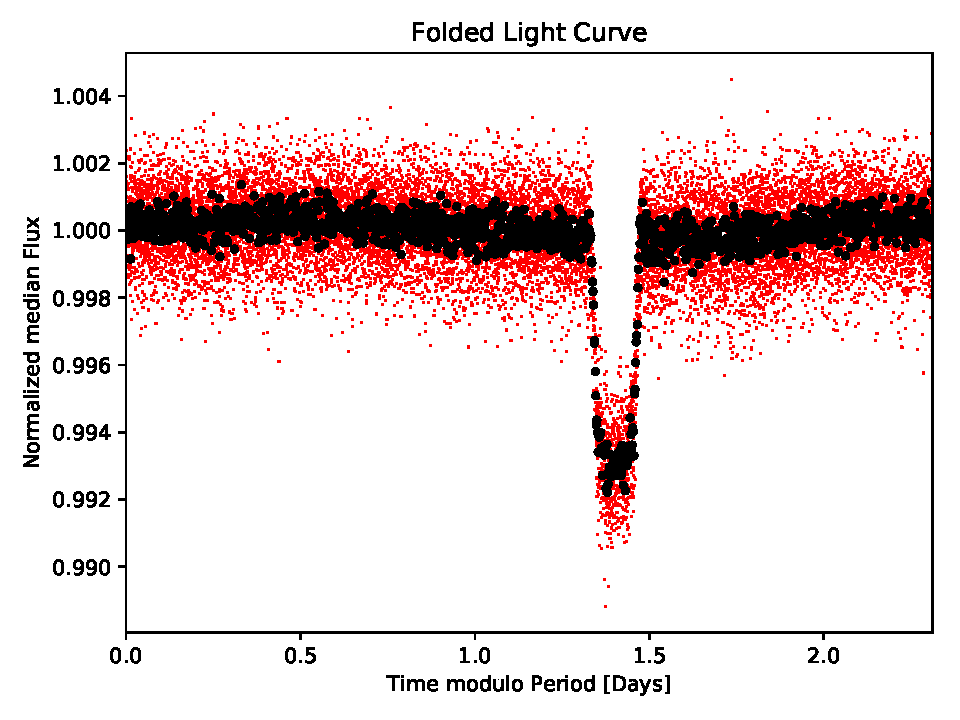
\includegraphics[width=0.9\textwidth]{../figures/2019-1-16_13:47:28_Folded_TIC25375553.pdf}
\end{frame}

\subsection{No Signal?}

\begin{frame}
\frametitle{No signal?}
\centering
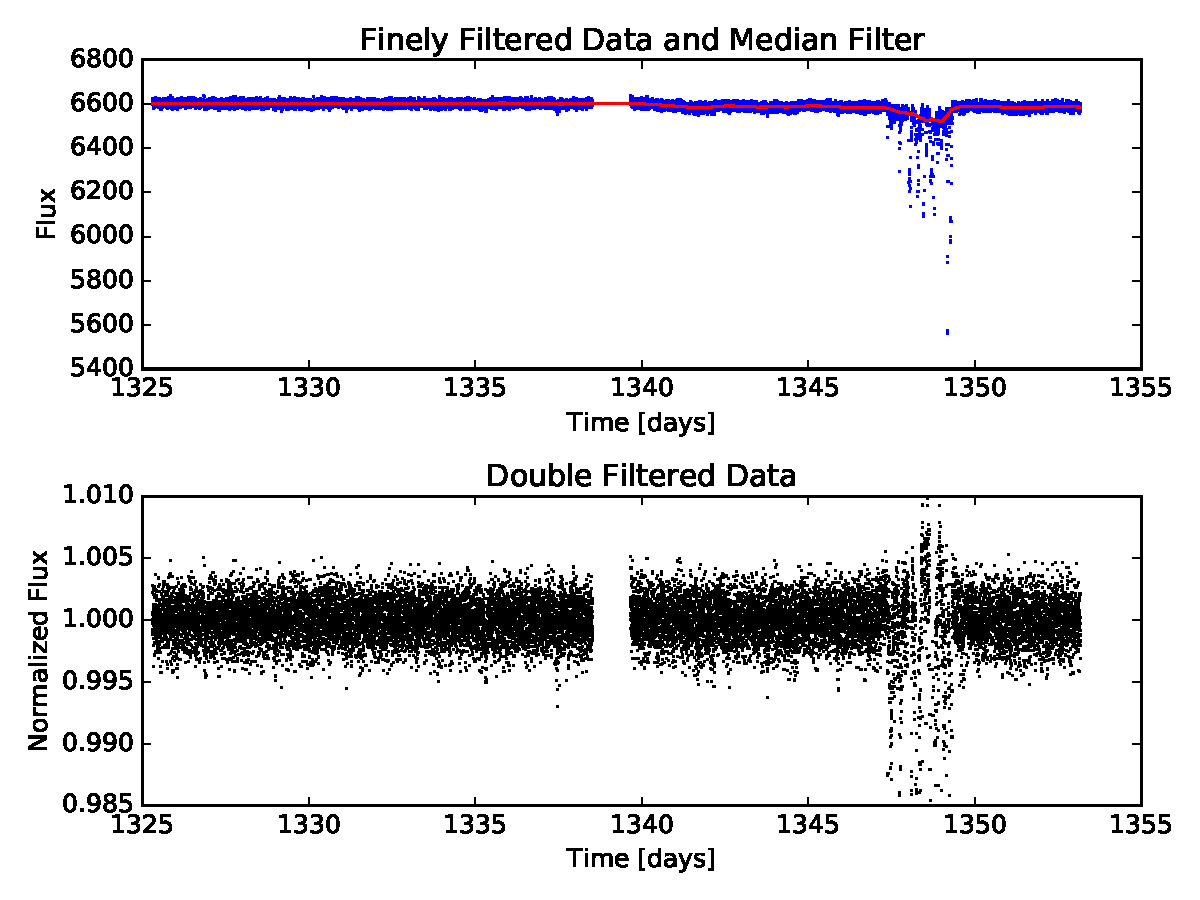
\includegraphics[width=0.9\textwidth]{../figures/2019-1-15_16:2:14_normcurve_lightcurve_TIC89020549.pdf}
\end{frame}

\begin{frame}
\frametitle{No signal?}
\centering
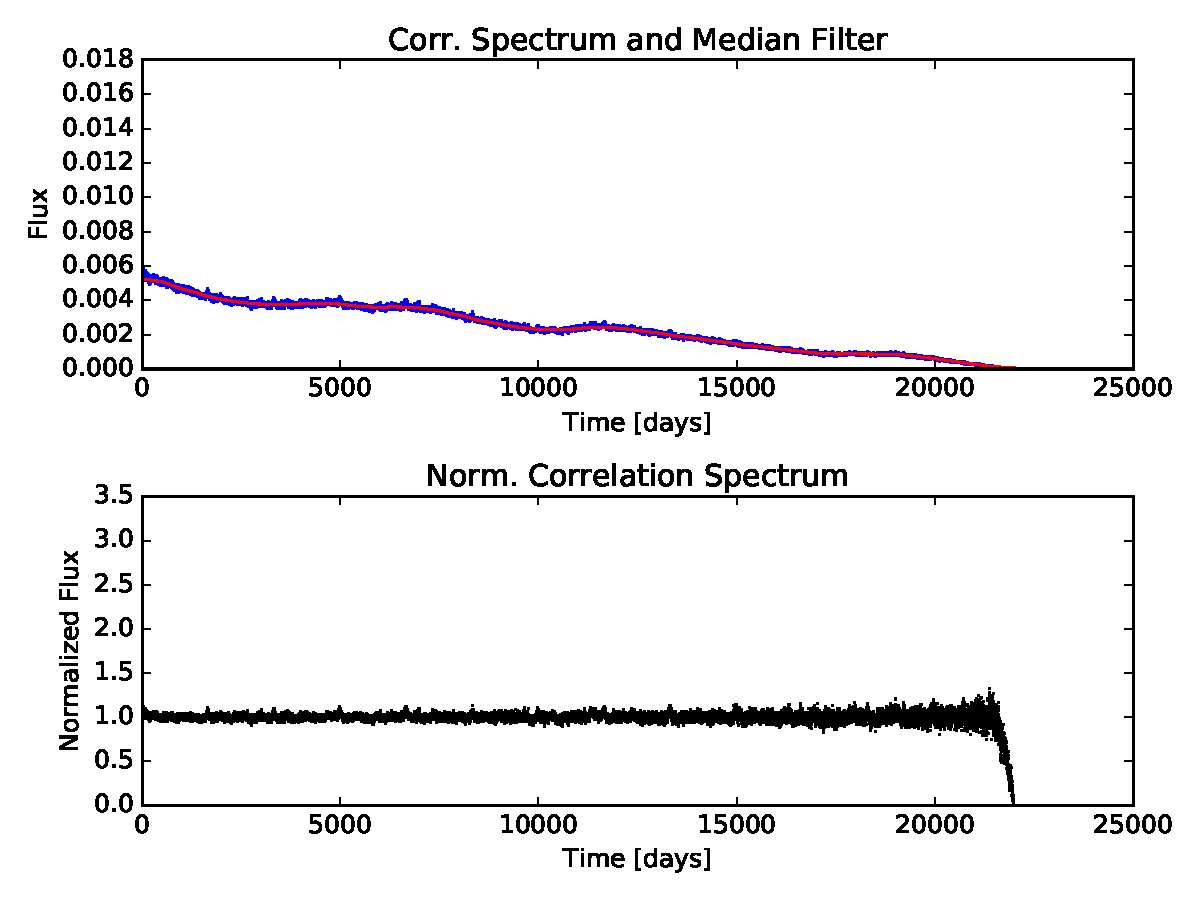
\includegraphics[width=0.9\textwidth]{../figures/2019-1-15_16:2:14_normcurve_correlation_TIC89020549.pdf}
\end{frame}

\begin{frame}
\frametitle{No signal?}
\centering
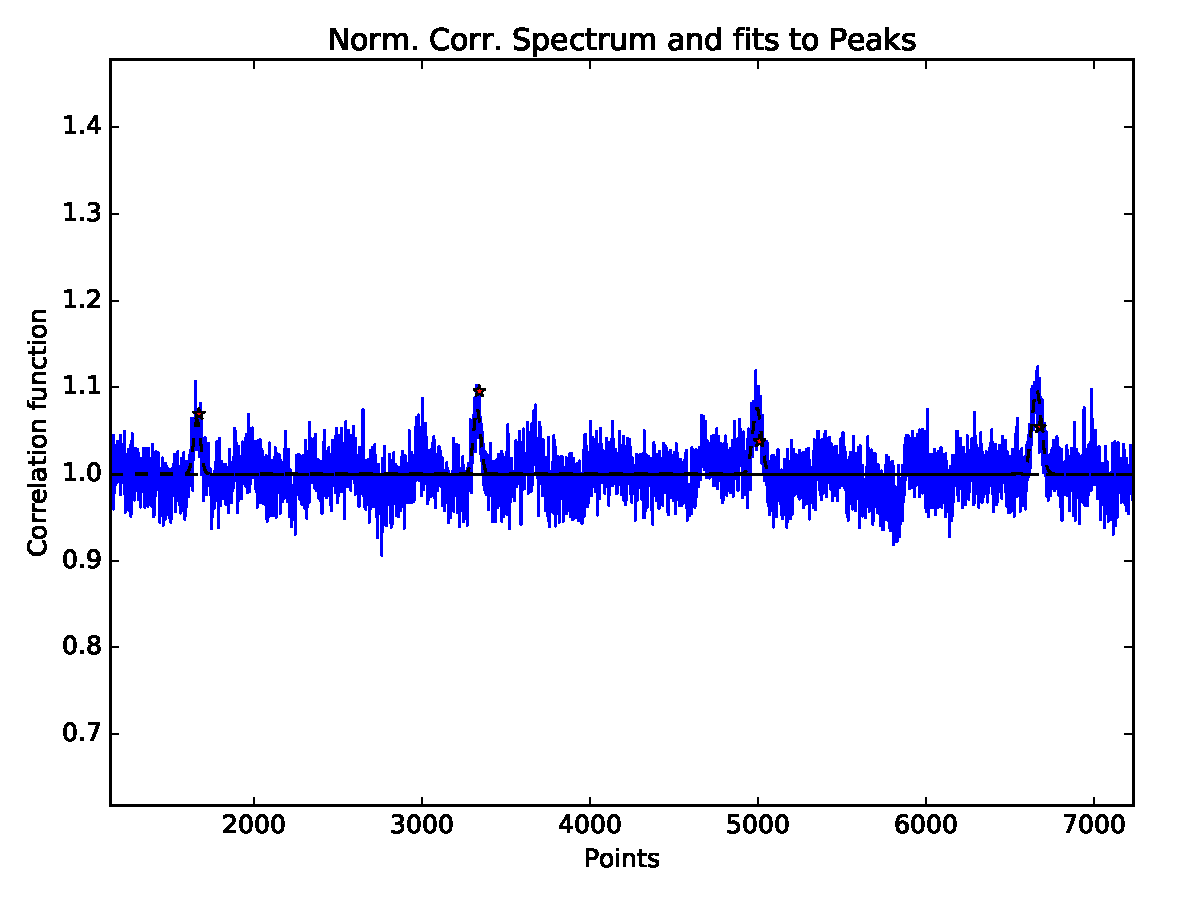
\includegraphics[width=0.9\textwidth]{../figures/Corr-spektrum_zoom.pdf}
\end{frame}

\begin{frame}
\frametitle{No signal?}
\centering
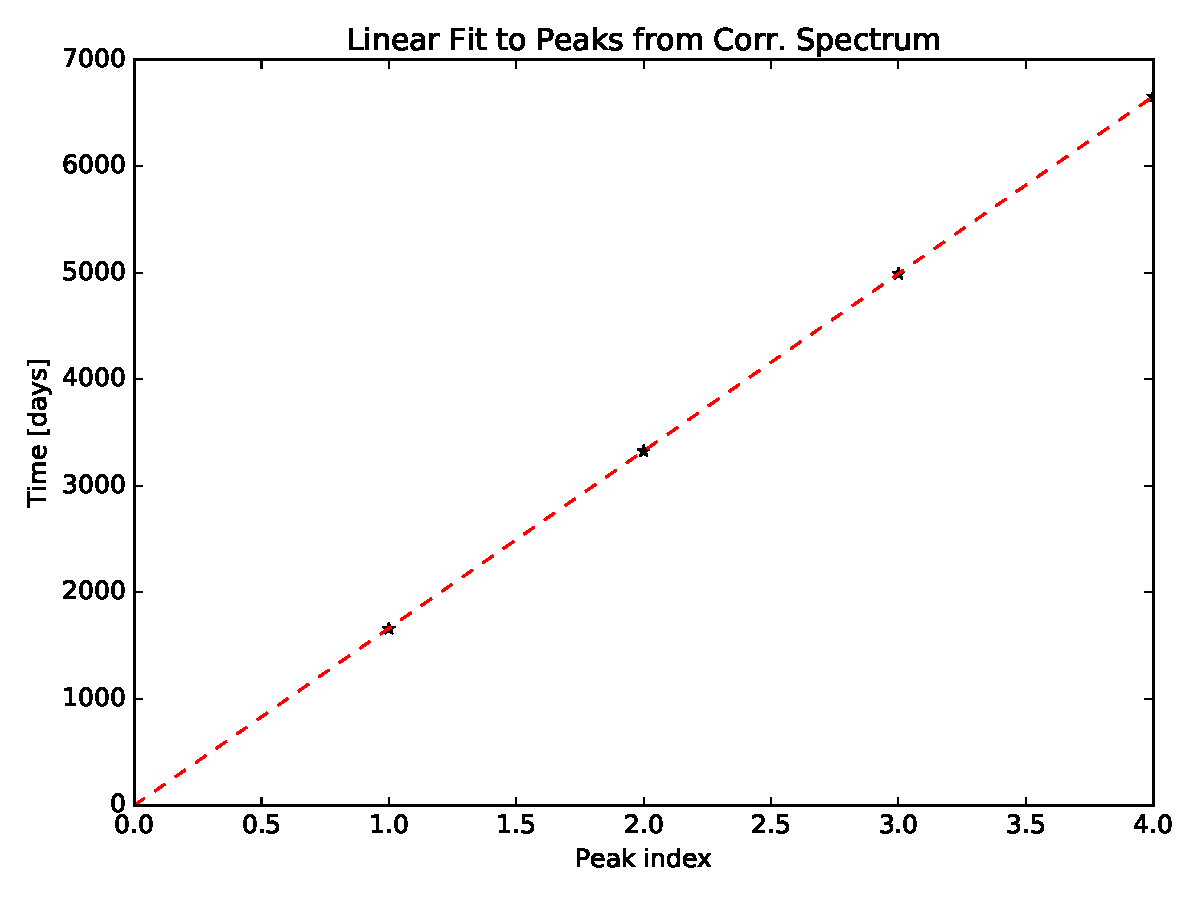
\includegraphics[width=0.9\textwidth]{../figures/2019-1-15_16:2:14_linear_fit_TIC89020549.pdf}
\end{frame}

\begin{frame}
\frametitle{No signal?}
\centering
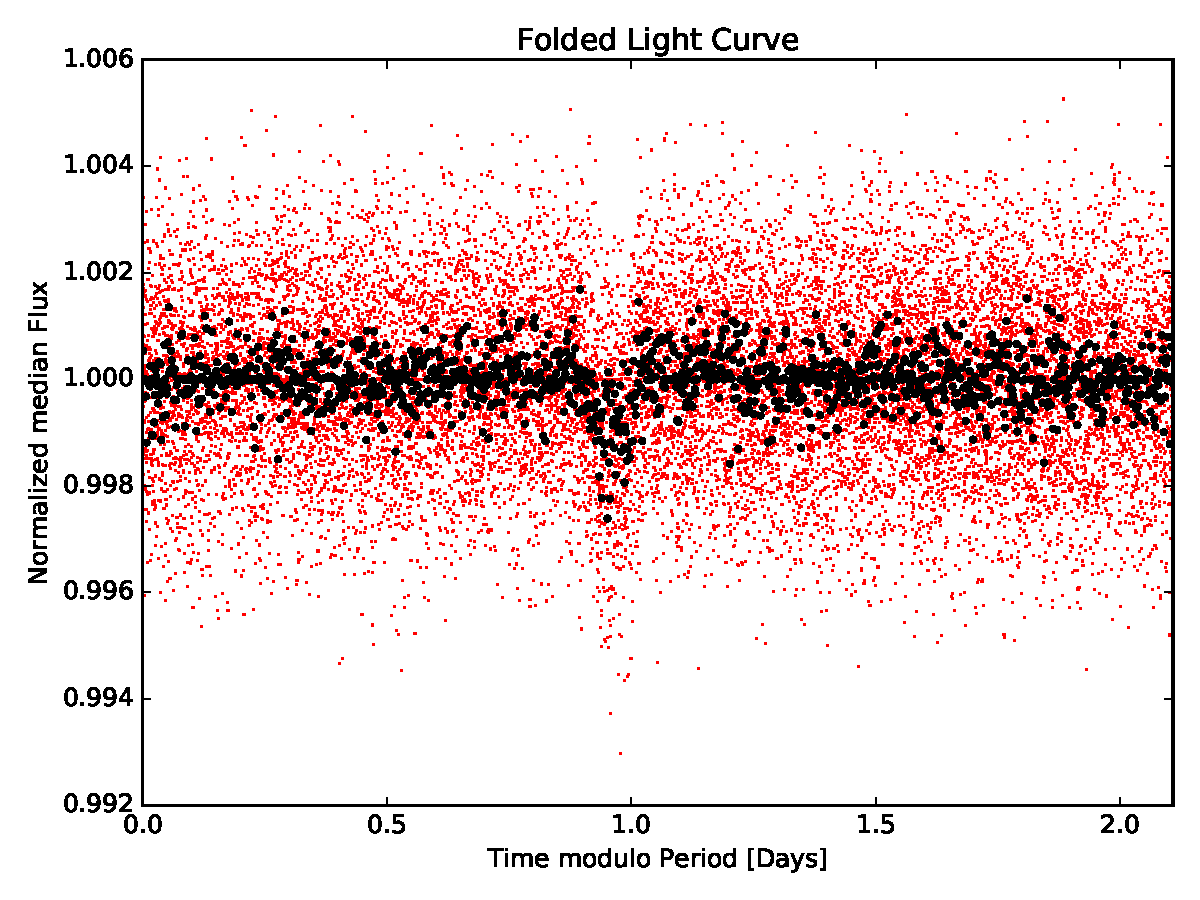
\includegraphics[width=0.9\textwidth]{../figures/2019-1-15_16:2:14_Folded_TIC89020549.pdf}
\end{frame}

\begin{frame}
\frametitle{Mandel-Agol Transit Model}
\begin{columns}
	\column{0.5\textwidth}
	\begin{itemize}
		\item Analytical Model
		\item Limb Darkening, Quadratic
		\item Parameters:
		\begin{itemize}
			\item Radius Ratio, $ R_p/R_{\star} = \sqrt{D} $
			\item Semimajor axis, $ a/R_{\star} $
			\item Inclination
			\item Period
			\item Time of Periapsis Passage, $ \tau $
			\item Orbital eccentricity
		\end{itemize}
	\end{itemize}
	\column{0.5\textwidth}
	Not used:
	\begin{itemize}
		\item Flux ratio between star and stellar companion
		\item Longitude of ascending node
		\item Argument of periapsis
	\end{itemize}
\end{columns}
\end{frame}

\begin{frame}
	\frametitle{MCMC-fitting, Marcov Chain Monte Carlo}
	\begin{columns}
		\column{0.5\textwidth}
		In:
		\begin{itemize}
			\item Intial guesses, intervals, and step sizes
			\item Prior distribution
			\item Number of iterations
			\item Burn, number of iterations excluded
		\end{itemize}
		
		Out:
		\begin{itemize}
			\item Trace
			\item Posterior distribution
			\item Guess for best value of parameter
		\end{itemize}
		\column{0.5\textwidth}
		\centering
		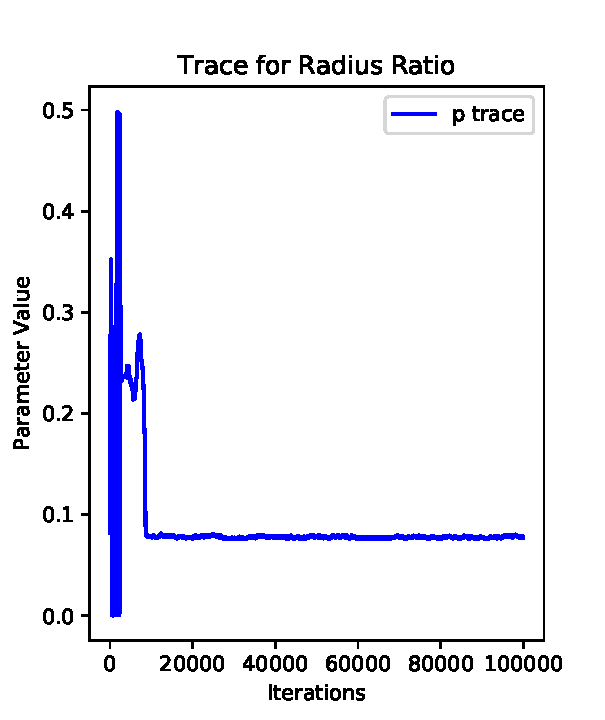
\includegraphics[width=\columnwidth]{../figures/Trace_for_radius_Ratio.pdf}
	\end{columns}
	
\end{frame}

\begin{frame}
	\frametitle{Mandel-Agol Transit Model}
	Initial Guesses:
	\begin{itemize}
		\item Period set fixed to calculated value
		\item Radius ratio from minimum flux value
		\item Inclination, $ 80 \degree$
		\item $ \tau $, mid point of time axis
		\item Eccentricity, $ 0.10 $
	\end{itemize}
\end{frame}


\begin{frame}
\frametitle{MCMC-fit}
\centering
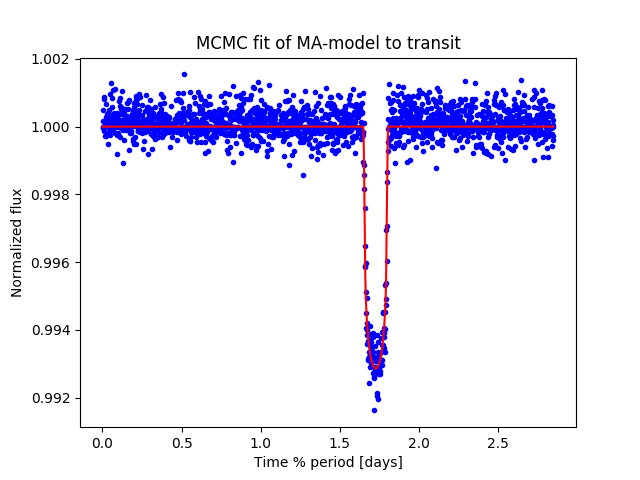
\includegraphics[width=0.9\textwidth]{../figures/MCMC_fit0.png}
\end{frame}

\begin{frame}
	\frametitle{Improvements}
	\begin{itemize}
		\item Access to more computational power
		\item Finding limb darkening guesses from stellar parameters
		
		
	\end{itemize}
\end{frame}


\end{document}